\documentclass[12pt]{article}
%\usepackage{bbm}
\usepackage{amsmath}
\usepackage{amsfonts}
\usepackage{graphicx}
\begin{document}
\section{answer email questions}
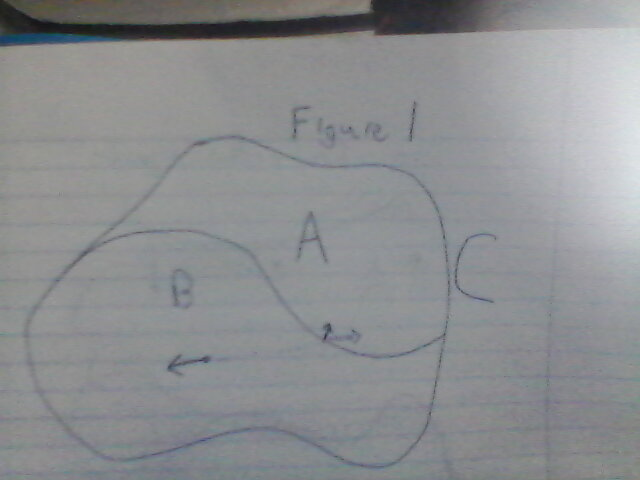
\includegraphics[width=120mm]{figure1.jpg}\\
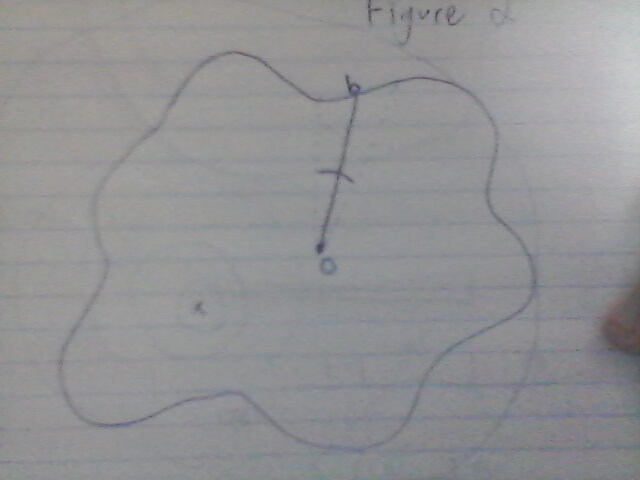
\includegraphics[width=120mm]{figure2.jpg}\\
I hope this clarifies all of the questions you asked me
My approach starts by first constructing a monte carlo method which equals the probability of the sequence under consideration, chosen randomly to be in this minibatch, of being chosen.  
With a region like I drew in figure 2, I acquire a point $p_0$ in the latent space by passing a point I know maps on to the chosen piece of categorical data inverse through the network. The point is the dot with a 0 by it in the figure. The region represents the area in the latent space that when passed forwards through the network maps on to the same piece of categorical data as the central point. The mapping on to categorical data from the output space will normally be argmax. \\
My goal is now to measure the probability enclosed in this region. For this to be defined, I need to have a probability distribution over the latent space. I chose the multivaraite gaussian distribution, with a standard deviation of 1 and mean of 0 and an identity covariance matrix. I depicted this as an X with rings of probablility around it in figure 2. The probablitiy enclosed in the region is the probability of that piece of categorical data being generated and that was what I refered to in the email. 
\\
My procedure for the monte carlo integral goes as follows. 
\\
I start by sampling a vector $v$ of spherical noise, and measure the euclidean distance to the boundary of the region using a root finding algorithm. I represent the distance as $b$ Because I am using spherical noise, I model the vector to the boundary as an infinitesimally narrow cone. I depicted this using the dashed lines is figure 2. 
The expression for the probability estimate from that vector in dimention $d$ is $$q=\int_0^b pdf of gaussian*area ofslice of cone *jacobian determinant = $$ $$ \int_0^b {\frac{1}{\sqrt{2*\pi}}}^d e^{-|(p_0+v*x)|^2} x^{d-1}*A  Unit Hypershell(d-1) \mathop{dx}$$
The area of the unit hypershell is the jacobian determinant because spherical noise is being used. I have verified in my code that this expression gives a probability of 1 starting from 0 to infinity in dimentions up to 100. \\
The NLL loss therefore is $-log(\mathbb{E}[q])$ By jensens inequality, because the negative logarithm is convex, I minimize the upper bound of $\mathbb{E}[-log(q)]$
I use the gradients of this expression to produce the gradients I showed in figure 1 and becuase this model is bijective, I can backpropagate them through the inverse of the model and use this to minimize loss. I have found this is a fairly loose upper bound, but it uncovered correct odds on a couple of toy problems I tried it on. For coding this, I used the logsumexp trick to stabilly estimate the integral. \\
The regions in the latent space mapping on to a given sequence, are as you noted, almost certainly not convex. I would like to show that bisection algorithm produces a higher loss for a non-convex region than for a convex region. Because probability is always greater than 1, the NLL is a decreasing function of the distance to the located boundary. I believe that would make the lowest loss configuration have every region be convex, but I am not sure how to prove that. Could you help?
\end{document}